\documentclass[a4paper]{report}
% Some basic packages
\usepackage[utf8]{inputenc}
\usepackage[T1]{fontenc}
\usepackage{textcomp}
\usepackage[english]{babel}
\usepackage{url}
\usepackage{graphicx}
\usepackage{float}
\usepackage{booktabs}
\usepackage{enumitem}

\pdfminorversion=7

% Don't indent paragraphs, leave some space between them
\usepackage{parskip}

% Hide page number when page is empty
\usepackage{emptypage}
\usepackage{subcaption}
\usepackage{multicol}
\usepackage{xcolor}

% Other font I sometimes use.
% \usepackage{cmbright}

% Math stuff
\usepackage{amsmath, amsfonts, mathtools, amsthm, amssymb}
% Fancy script capitals
\usepackage{mathrsfs}
\usepackage{cancel}
% Bold math
\usepackage{bm}
% Some shortcuts
\newcommand\N{\ensuremath{\mathbb{N}}}
\newcommand\R{\ensuremath{\mathbb{R}}}
\newcommand\Z{\ensuremath{\mathbb{Z}}}
\renewcommand\O{\ensuremath{\emptyset}}
\newcommand\Q{\ensuremath{\mathbb{Q}}}
\newcommand\C{\ensuremath{\mathbb{C}}}
\renewcommand\L{\ensuremath{\mathcal{L}}}

% Package for Petri Net drawing
\usepackage[version=0.96]{pgf}
\usepackage{tikz}
\usetikzlibrary{arrows,shapes,automata,petri}
\usepackage{tikzit}
\input{petri_nets_style.tikzstyles}

% Easily typeset systems of equations (French package)
\usepackage{systeme}

% Put x \to \infty below \lim
\let\svlim\lim\def\lim{\svlim\limits}

%Make implies and impliedby shorter
\let\implies\Rightarrow
\let\impliedby\Leftarrow
\let\iff\Leftrightarrow
\let\epsilon\varepsilon

% Add \contra symbol to denote contradiction
\usepackage{stmaryrd} % for \lightning
\newcommand\contra{\scalebox{1.5}{$\lightning$}}

% \let\phi\varphi

% Command for short corrections
% Usage: 1+1=\correct{3}{2}

\definecolor{correct}{HTML}{009900}
\newcommand\correct[2]{\ensuremath{\:}{\color{red}{#1}}\ensuremath{\to }{\color{correct}{#2}}\ensuremath{\:}}
\newcommand\green[1]{{\color{correct}{#1}}}

% horizontal rule
\newcommand\hr{
    \noindent\rule[0.5ex]{\linewidth}{0.5pt}
}

% hide parts
\newcommand\hide[1]{}

% si unitx
\usepackage{siunitx}
\sisetup{locale = FR}

% Environments
\makeatother
% For box around Definition, Theorem, \ldots
\usepackage{mdframed}
\mdfsetup{skipabove=1em,skipbelow=0em}
\theoremstyle{definition}
\newmdtheoremenv[nobreak=true]{definitie}{Definitie}
\newmdtheoremenv[nobreak=true]{eigenschap}{Eigenschap}
\newmdtheoremenv[nobreak=true]{gevolg}{Gevolg}
\newmdtheoremenv[nobreak=true]{lemma}{Lemma}
\newmdtheoremenv[nobreak=true]{propositie}{Propositie}
\newmdtheoremenv[nobreak=true]{stelling}{Stelling}
\newmdtheoremenv[nobreak=true]{wet}{Wet}
\newmdtheoremenv[nobreak=true]{postulaat}{Postulaat}
\newmdtheoremenv{conclusie}{Conclusie}
\newmdtheoremenv{toemaatje}{Toemaatje}
\newmdtheoremenv{vermoeden}{Vermoeden}
\newtheorem*{herhaling}{Herhaling}
\newtheorem*{intermezzo}{Intermezzo}
\newtheorem*{notatie}{Notatie}
\newtheorem*{observatie}{Observatie}
\newtheorem*{exe}{Exercise}
\newtheorem*{opmerking}{Opmerking}
\newtheorem*{praktisch}{Praktisch}
\newtheorem*{probleem}{Probleem}
\newtheorem*{terminologie}{Terminologie}
\newtheorem*{toepassing}{Toepassing}
\newtheorem*{uovt}{UOVT}
\newtheorem*{vb}{Voorbeeld}
\newtheorem*{vraag}{Vraag}

\newmdtheoremenv[nobreak=true]{definition}{Definition}
\newtheorem*{eg}{Example}
\newtheorem*{notation}{Notation}
\newtheorem*{previouslyseen}{As previously seen}
\newtheorem*{remark}{Remark}
\newtheorem*{note}{Note}
\newtheorem*{problem}{Problem}
\newtheorem*{observe}{Observe}
\newtheorem*{property}{Property}
\newtheorem*{intuition}{Intuition}
\newmdtheoremenv[nobreak=true]{prop}{Proposition}
\newmdtheoremenv[nobreak=true]{theorem}{Theorem}
\newmdtheoremenv[nobreak=true]{corollary}{Corollary}

% End example and intermezzo environments with a small diamond (just like proof
% environments end with a small square)
\usepackage{etoolbox}
\AtEndEnvironment{vb}{\null\hfill$\diamond$}%
\AtEndEnvironment{intermezzo}{\null\hfill$\diamond$}%
% \AtEndEnvironment{opmerking}{\null\hfill$\diamond$}%

% Fix some spacing
% http://tex.stackexchange.com/questions/22119/how-can-i-change-the-spacing-before-theorems-with-amsthm
\makeatletter
\def\thm@space@setup{%
  \thm@preskip=\parskip \thm@postskip=0pt
}


% Exercise 
% Usage:
% \exercise{5}
% \subexercise{1}
% \subexercise{2}
% \subexercise{3}
% gives
% Exercise 5
%   Exercise 5.1
%   Exercise 5.2
%   Exercise 5.3
\newcommand{\exercise}[1]{%
    \def\@exercise{#1}%
    \subsection*{Exercise #1}
}

\newcommand{\subexercise}[1]{%
    \subsubsection*{Exercise \@exercise.#1}
}


% \lecture starts a new lecture (les in dutch)
%
% Usage:
% \lecture{1}{di 12 feb 2019 16:00}{Inleiding}
%
% This adds a section heading with the number / title of the lecture and a
% margin paragraph with the date.

% I use \dateparts here to hide the year (2019). This way, I can easily parse
% the date of each lecture unambiguously while still having a human-friendly
% short format printed to the pdf.

\usepackage{xifthen}
\def\testdateparts#1{\dateparts#1\relax}
\def\dateparts#1 #2 #3 #4 #5\relax{
    \marginpar{\small\textsf{\mbox{#1 #2 #3 #5}}}
}

\def\@lecture{}%
\newcommand{\lecture}[3]{
    \ifthenelse{\isempty{#3}}{%
        \def\@lecture{Lecture #1}%
    }{%
        \def\@lecture{Lecture #1: #3}%
    }%
    \subsection*{\@lecture}
    \marginpar{\small\textsf{\mbox{#2}}}
}



% These are the fancy headers
\usepackage{fancyhdr}
\pagestyle{fancy}

% LE: left even
% RO: right odd
% CE, CO: center even, center odd
% My name for when I print my lecture notes to use for an open book exam.
% \fancyhead[LE,RO]{Gilles Castel}

\fancyhead[RO,LE]{\@lecture} % Right odd,  Left even
\fancyhead[RE,LO]{}          % Right even, Left odd

\fancyfoot[RO,LE]{\thepage}  % Right odd,  Left even
\fancyfoot[RE,LO]{}          % Right even, Left odd
\fancyfoot[C]{\leftmark}     % Center

\makeatother




% Todonotes and inline notes in fancy boxes
\usepackage{todonotes}
\usepackage{tcolorbox}

% Make boxes breakable
\tcbuselibrary{breakable}

% Verbetering is correction in Dutch
% Usage: 
% \begin{verbetering}
%     Lorem ipsum dolor sit amet, consetetur sadipscing elitr, sed diam nonumy eirmod
%     tempor invidunt ut labore et dolore magna aliquyam erat, sed diam voluptua. At
%     vero eos et accusam et justo duo dolores et ea rebum. Stet clita kasd gubergren,
%     no sea takimata sanctus est Lorem ipsum dolor sit amet.
% \end{verbetering}
\newenvironment{verbetering}{\begin{tcolorbox}[
    arc=0mm,
    colback=white,
    colframe=green!60!black,
    title=Opmerking,
    fonttitle=\sffamily,
    breakable
]}{\end{tcolorbox}}

% Noot is note in Dutch. Same as 'verbetering' but color of box is different
\newenvironment{noot}[1]{\begin{tcolorbox}[
    arc=0mm,
    colback=white,
    colframe=white!60!black,
    title=#1,
    fonttitle=\sffamily,
    breakable
]}{\end{tcolorbox}}




% Figure support as explained in my blog post.
\usepackage{import}
\usepackage{xifthen}
\usepackage{pdfpages}
\usepackage{transparent}
\newcommand{\incfig}[1]{%
    \def\svgwidth{\columnwidth}
    \import{./figures/}{#1.pdf_tex}
}

% Fix some stuff
% %http://tex.stackexchange.com/questions/76273/multiple-pdfs-with-page-group-included-in-a-single-page-warning
\pdfsuppresswarningpagegroup=1


% My name
\author{Bruno M. Pacheco}

 
\begin{document}
 
\title{Controle de Temperatura e Nível de Tanque\\Componentes e Circuitos}
\author{Bruno M. Pacheco (16100865) \\
DAS5151 - Instrumentação em Controle}
 
\maketitle

\section*{Projeto Mecânico}

A planta deste projeto consiste em um tanque cilíndrico no qual deseja-se realizar um controle automático de temperatura ao longo do líquido e um controle manual de nível através da vazão de entrada e saída. O esquemático da montagem pode ser observado na imagem abaixo.

\begin{figure}[H]
    \centering
    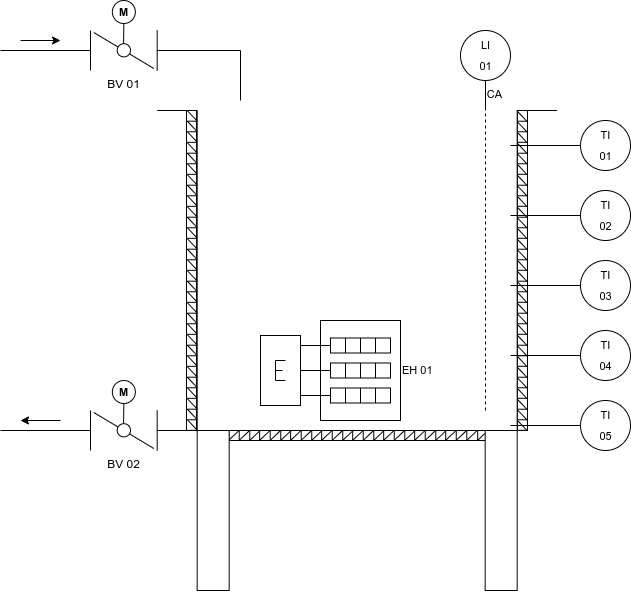
\includegraphics[width=0.8\textwidth]{figures/tank.png}
\end{figure}

Como se pode observar, o fluído entra no tanque pela sua superfície superior e é extraído de sua base através de válvulas borboleta (BV 01 e 02). Além disso, o aquecimento é feito na base, através de um aquecedor elétrico (EH 01), bastante próximo da saída. Também é de destaque o isolamento térmico, marcado pela área hachurada, restando somente a troca de calor através da superfície do líquido como fonte de perdas térmicas significantes.

5 transdutores de temperatura (TI 01 até 05) foram projetados ao longo da parede do tanque, garantindo sensoriamento mais granular no conteúdo. Também, um transdutor de nível (LI 01) é essencial para o controle manual.

O modelo da planta (propagação térmica e dinâmica do fluído) segue o desenvolvido no trabalho de LabVIEW.

\section*{Componentes}

A relação geral dos componentes pode ser observada na tabela abaixo.

\begin{table}[H]
\begin{tabular}{l|l|l}
\textbf{Código} & \textbf{Nome}                   & \textbf{Componente} \\ \hline
EH 01           & Aquecedor elétrico              & TMT04014            \\ \hline
BV 01/02        & Válvula de entrada              & D6100N+DR24A-SR-5   \\ \hline
LI 01           & Transdutor capacitivo de nível  & LSP-050.1.500       \\ \hline
TI 01/.../05    & Transdutor de temperatura PT100 & TRA-C61\footnotemark \\ \hline
\end{tabular}
\end{table}

\footnotetext{\url{https://pdf.directindustry.com/pdf/krohne-messtechnik/optitemp-tra-h6x-c6x/5863-961839.html}}

Todas as simulações de circuitos expostas a seguir foram feitas no LTSpice com modelos dos componentes reais sempre quie possível.

\subsection*{Atuadores}

\subsubsection*{Aquecedor elétrico}

O aquecedor elétrico utilizado será o aquecedor de imersão TMT04014. Ele possui um acionamento ON/OFF direto na rede. Modelado como uma carga puramente resistiva, seu acionamento foi projetado através de uma combinação de um opto-DIAC (MOC3023) e um TRIAC (2N5446) em cascata, garantindo isolamento entre o sistema de controle e a rede elétrica. O resultado da simulação desse circuito pode ser observada na figura abaixo.

\begin{figure}[H]
    \centering
    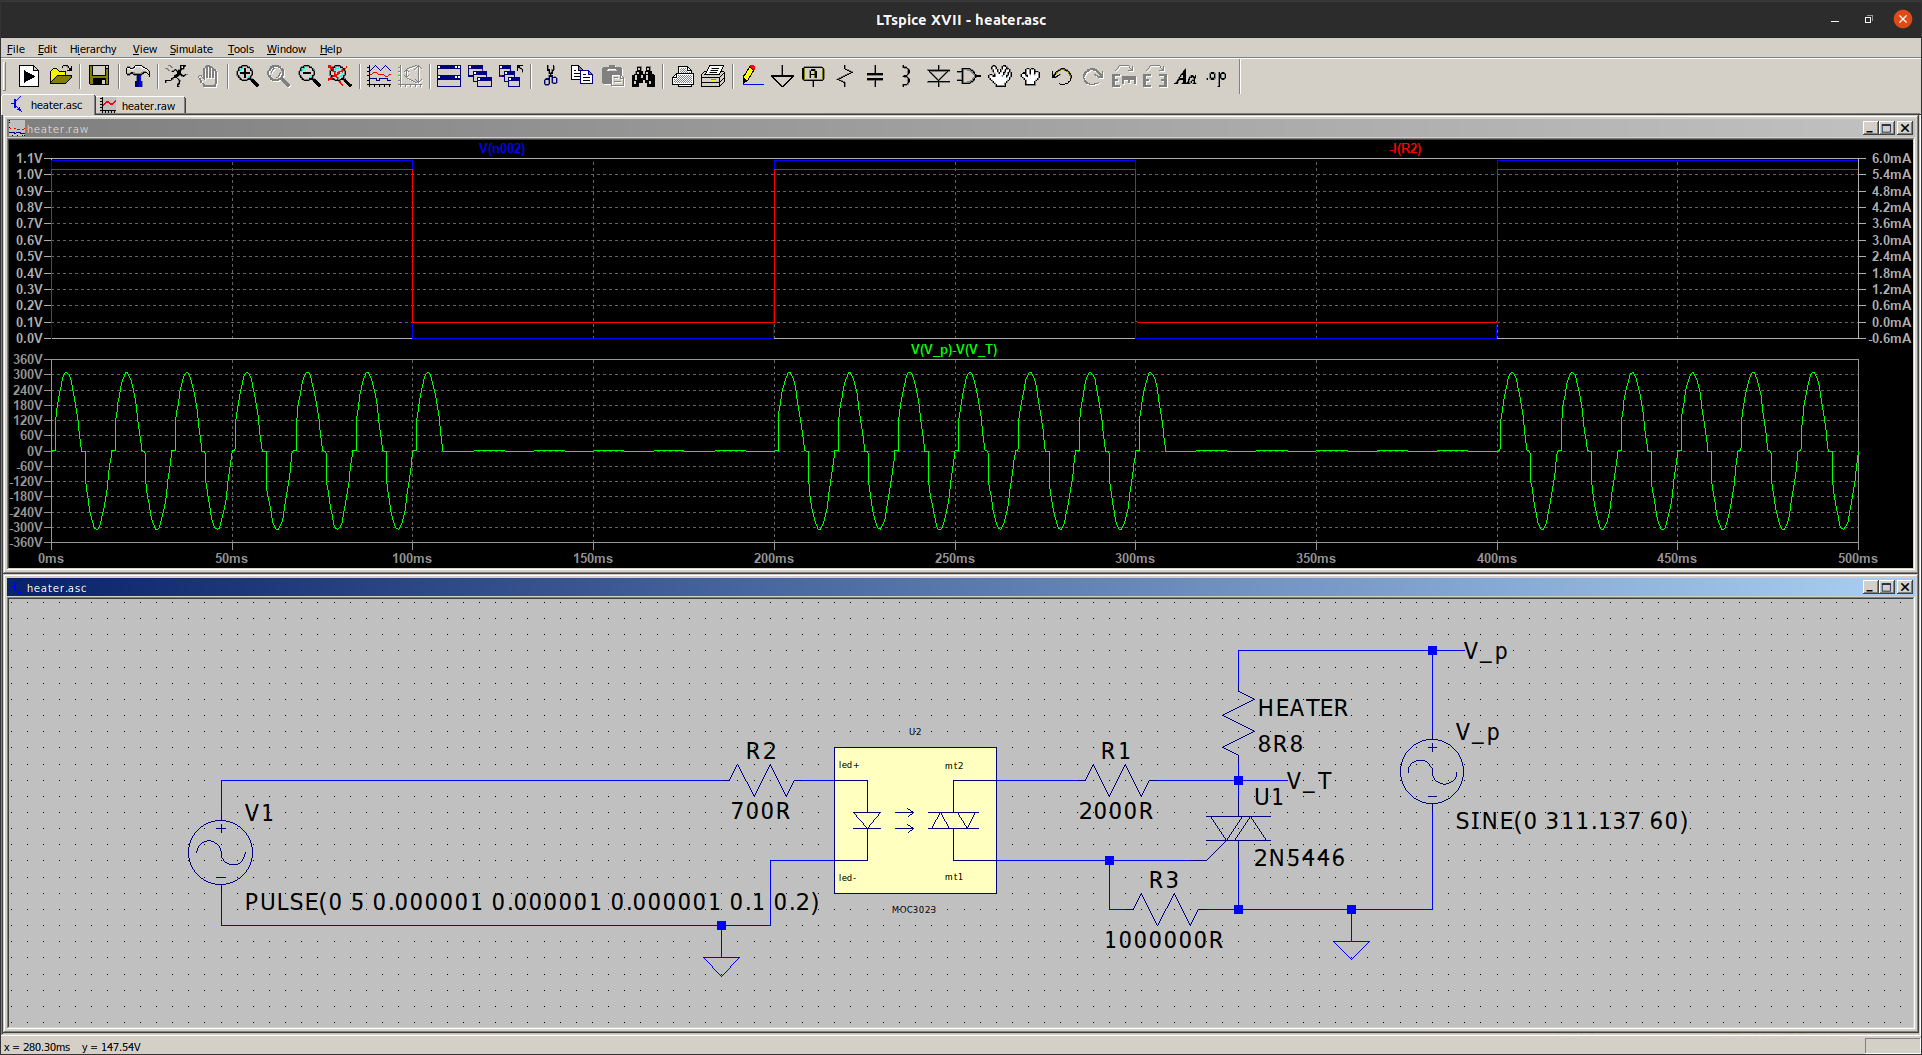
\includegraphics[width=0.8\textwidth]{figures/sym_heater.png}
\end{figure}

Como pode ser observado, o sinal de controle (no gráfico, \emph{V(n002)}, em azul) foi convertido em acionamento da carga que representa o aquecedor com sucesso sem consumir grande potência do sistema de acionamento.

\subsubsection*{Válvulas}

A solução encontrada tanto para o controle do fluxo de líquido é o conjunto de atuador e válvula da Belimo. Em particular, projetou-se o uso dos atuadores rotacionais da linha DR24A e válvulas borboleta da linha D6..N. Para realizar o acionamento, será utilizado um LM741 para amplificar o sinal do sistema de controle para a faixa de operação do atuador rotacional (ganho 2). O resultado pode ser observado na figura abaixo.

\begin{figure}[H]
    \centering
    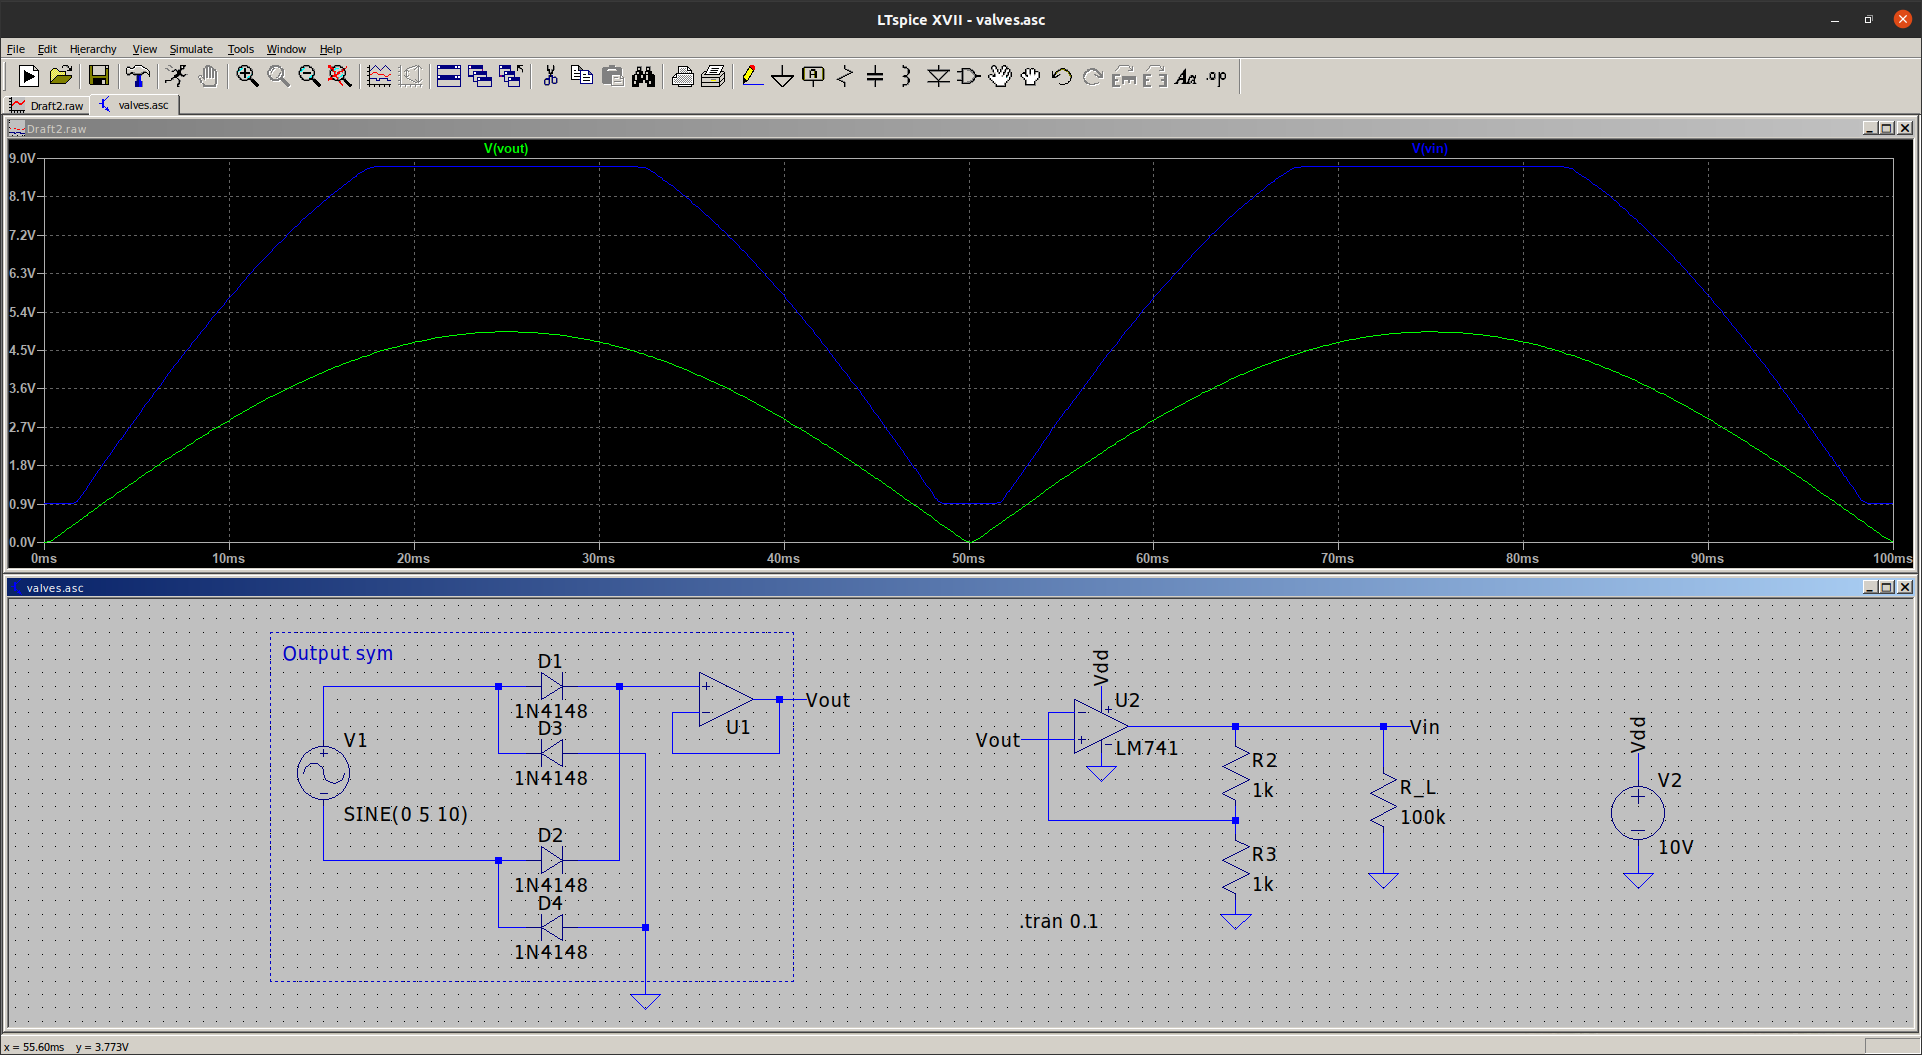
\includegraphics[width=0.8\textwidth]{figures/sym_valve.png}
\end{figure}

Destaca-se que o bloco \emph{Output sym} é utilizado somente para simular um sinal de controle e não faz parte do projeto.

\subsection*{Transdutores}

\subsubsection*{Temperatura}

Para fazer o monitoramento da temperatura foram escolhidos os transdutores da KROHNE da linha TRA-H6X/-C6X, que seguem o padrão PT100. Para a transmissão do sinal, projetou-se um cabo manga 4x26 AWG com blindagem. Para evitar o uso de uma fonte de corrente, o circuito para aquisição de sinal consiste em um divisor resistivo e uma medição a 3 fios. Além disso, para que não seja necessária uma fonte simétrica, seguiu-se as recomendações de projeto da Texas Instruments para amplificadores operacionais com fonte única (arquivo anexo).

Dessa forma, empregou-se um LM358 (próprio para utilização com alimentação única) em um arranjo próprio para amplificar o sinal e controlar o \emph{offset}. Assim, condicionou-se o sinal para que a faixa de operação desejada (0 a 100ºC) seja mapeada na faixa de 1 a 4 V, se mantendo fora dos limites de operação do amplificador operacional. O resultado da simulação pode ser visto na figura abaixo. Destaca-se que cada linha no gráfico é uma temperatura de entrada, variando de 0 a 100ºC em intervalos de 20ºC.

\begin{figure}[H]
    \centering
    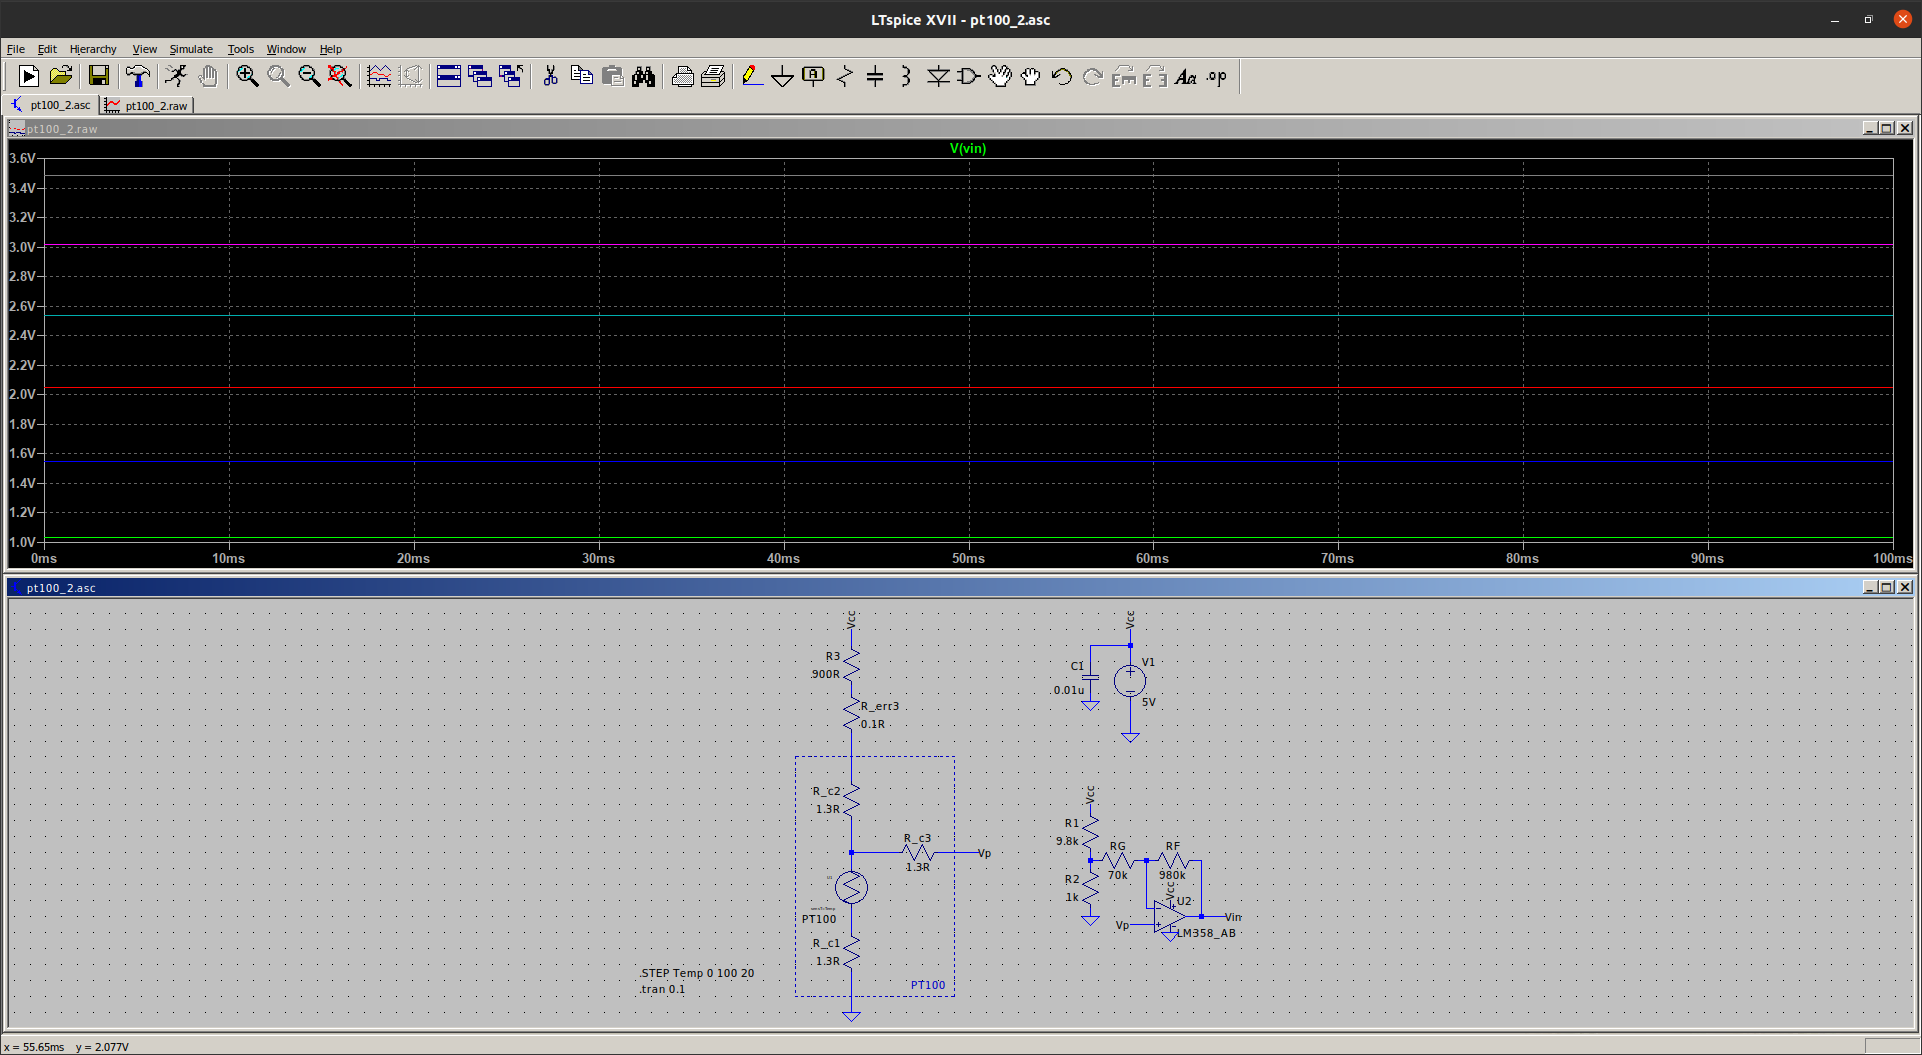
\includegraphics[width=0.8\textwidth]{figures/sym_pt100.png}
\end{figure}

\subsubsection*{Nível}

O sensoriamento do nível foi projetado em cima do transdutor capacitivo da linha LSP 05X, da Baumer. Sua saída é na forma de uma fonte de corrente, portanto, foi projetado um circuito de sensoriamento com um resistor dentro das suas capacidades de carga e um seguidor de tensão utilizando um LM358 para acoplar ao sistema de aquisição de dados. O resultado pode ser visto na figura abaixo.

\begin{figure}[H]
    \centering
    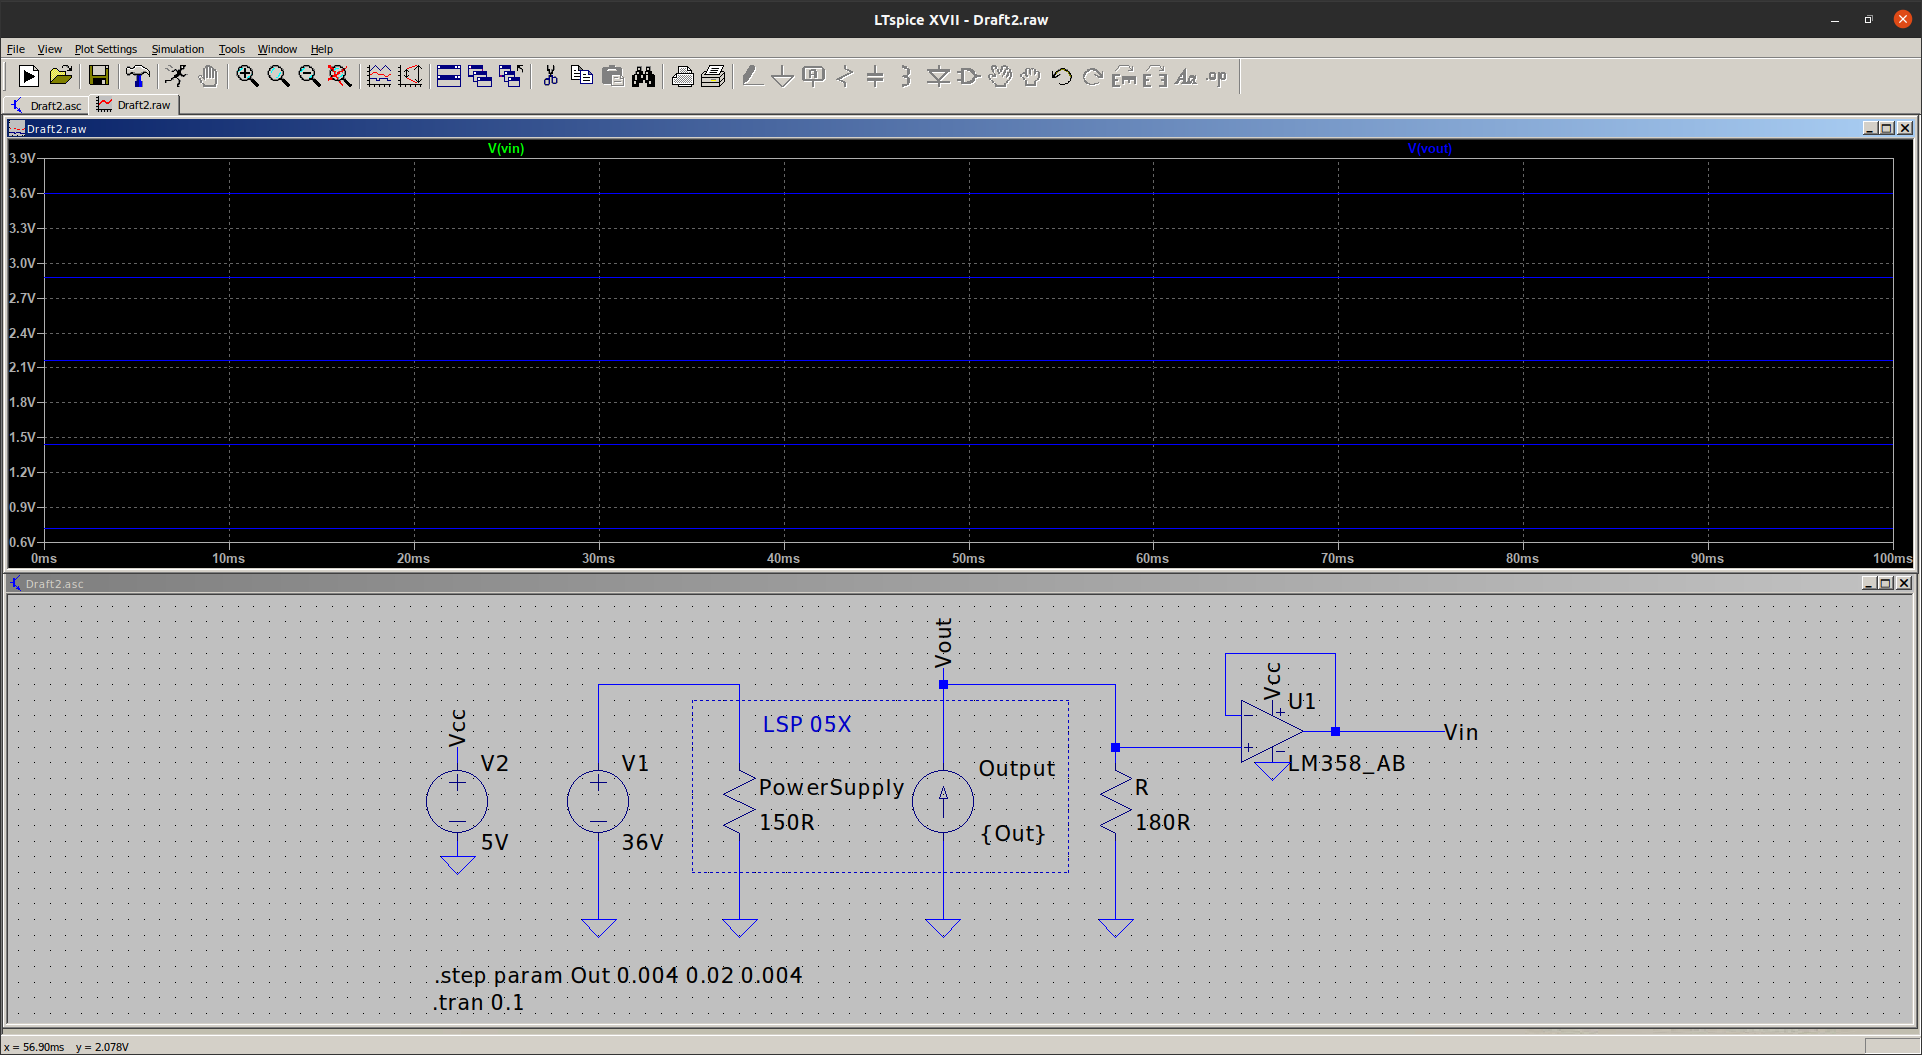
\includegraphics[width=0.8\textwidth]{figures/sym_level.png}
\end{figure}

\end{document}

